%iffalse
\let\negmedspace\undefined
\let\negthickspace\undefined
\documentclass[journal,12pt,onecolumn]{IEEEtran}
\usepackage{cite}
\usepackage{amsmath,amssymb,amsfonts,amsthm}
\usepackage{algorithmic}
\usepackage{multicol}
\usepackage{graphicx}
\usepackage{textcomp}
\usepackage{xcolor}
\usepackage{txfonts}
\usepackage{listings}
\usepackage{enumitem}
\usepackage{mathtools}
\usepackage{gensymb}
\usepackage{comment}
\usepackage[breaklinks=true]{hyperref}
\usepackage{tkz-euclide} 
\usepackage{listings}
\usepackage{gvv}                                        
%\def\inputGnumericTable{}                                 
\usepackage[latin1]{inputenc}                                
\usepackage{color}                                            
\usepackage{array}                                            
\usepackage{longtable}                                       
\usepackage{calc}                                             
\usepackage{multirow}                                         
\usepackage{hhline}                                           
\usepackage{ifthen}                                           
\usepackage{lscape}
\usepackage{tabularx}
\usepackage{array}
\usepackage{float}
\newtheorem{theorem}{Theorem}[section]
\newtheorem{problem}{Problem}
\newtheorem{proposition}{Proposition}[section]
\newtheorem{lemma}{Lemma}[section]
\newtheorem{corollary}[theorem]{Corollary}
\newtheorem{example}{Example}[section]
\newtheorem{definition}[problem]{Definition}
\newcommand{\BEQA}{\begin{eqnarray}}
\newcommand{\EEQA}{\end{eqnarray}}
\newcommand{\define}{\stackrel{\triangle}{=}}
\theoremstyle{remark}
\newtheorem{rem}{Remark}

% Marks the beginning of the document
\begin{document}
\bibliographystyle{IEEEtran}
\vspace{3cm}

\title{\textbf{NCERT 8 ex 13}}
\author{EE24BTECH11032- John Bobby}
\maketitle
\bigskip
\textbf{Question:} Prove that the curves $y^2=4x$ and $x^2=4y$ divide the area of the square bounded by $x=0$,$x=4$,$y=0$,$y=4$ into $3$ equal parts.\\
\textbf{Solution:}\\
\section{Theoretical Method}
The variables used in $y^2=4x$ are given below
\begin{table}[H]
    \centering
    \begin{tabular}[12pt]{ |c| c|} 
    \hline
    {Event} & {Denotation}\\ 
    \hline
    $A $ &  Student do pass in English \\
    \hline 
    $ A^\prime $ & Student does not pass in English\\
    \hline
    $ B $ & Student do pass in Hindi\\
    \hline   
    $ B^\prime $ & Student does not pass in English\\
    \hline
\end{tabular}

\end{table} 
The variables used in $x^2=4y$ are given below
\begin{table}[H]
    \centering
    \begin{tabular}{|l|c l|c l|}
    \hline
    & (a) & & (b) & \\
    \hline
    Postulate 2 & $A + 0 = A$ & & $A \cdot 1 = A$ & \\
    \hline
    Postulate 5 & $A + A' = 1$ & & $A
    \cdot A' = 0$ & \\
    \hline
    Theorem 1 & $A + A = A$ & & $A \cdot A = A$ & \\
    \hline
    Theorem 2 & $A + 1 = 1$ & & $A \cdot 0 = 0$ & \\
    \hline
    Theorem 3, involution & $(A')' = A$ & & - & \\
    \hline
    Postulate 3, commutative & $A + B = B + A$ & & $AB = BA$ & \\
    \hline
    Theorem 4, associative & $A + (B + C) = (A + B) + C$ & & $A(BC) = (AB)C$ & \\
    \hline
    Postulate 4, distributive & $A(B + C) = AB + AC$ & & $A + BC = (A + B)(A + C)$ & \\
    \hline
    Theorem 5, DeMorgan & $(A + B)' = A' B'$ & & $(AB)' = A' + B'$ & \\
    \hline
    Theorem 6, absorption & $A + AB = A$ & & $A(A + B) = A$ & \\
    \hline
\end{tabular}

\end{table} 
The point of intersection of the line with the parabolas is 
\begin{align}
    x_i = h + k_i m
\end{align}
where, $k_i$ is a constant and is calculated as follows:\\
\begin{align}
k_i = \frac{1}{m^\top Vm} \brak{-m^\top \brak{Vh + u} \pm \sqrt{\sbrak{m^\top \brak{Vh + u}}^2 - g\brak{h}\brak{m^\top Vm}}}.
\end{align}
Substituting the input parameters into $k_i$,\\
For the line $x=0$, $\vec{h}=\myvec{0 \\ 0}$, $\vec{m}=\myvec{0 \\ 0}$\\
For the function $y^2=4x$ we get $k=0$ Thus
$\vec{x}=\myvec{0 \\0}$\\
For the function $x^2=4y$ we get $k=0$ Thus
$\vec{x}=\myvec{0 \\0}$\\
Similarly, on repeating the same process for the line $x=4$ to each of the functions, we get the intersection points as $\myvec{4\\4}$ and $\myvec{4 \\4}$.\\

Area between $y^2=4x$ and $x^2=4y$ =$\int_{0}^{4} 2\sqrt{x} dx-\int_{0}^{4} \frac{x^2}{4} dx=\frac{32}{3}-\frac{16}{3}=\frac{16}{3}$\\
Area between $x^2=4y$ and $x=0$ and $x=4$=$\int_{0}^{4} 2\sqrt{x} dx=\frac{16}{3}$\\
Area between $y^2=4x$ and $y=0$ and $y=4$ =$\int_{0}^{4} \frac{y^2}{4} dy=\frac{16}{3}$\\
We can see that the $3$ areas are equal.\\
\section{Trapezoidal Method}
Using trapezoidal rule 
\begin{align*}
    \int_{a}^{b} f\brak{x}dx \approx \brak{b-a}\brak{\frac{f\brak{a}+f\brak{b}}{2}}
\end{align*}
Applying trapezoid rule for all values of $x$ between $0$ and $2\pi$\\
where $h$ is the step size 
\begin{align*}
    A&=\frac{1}{2}h\brak{y\brak{x_1}+y\brak{x_0}}+ \frac{1}{2}h\brak{y\brak{x_2}+y\brak{x_1}}+\dots+\frac{1}{2}h\brak{y\brak{x_n}+y\brak{x_{n-1}}}\\
\end{align*}
Let $A\brak{x_n}$ be the area enclosed by the curve $y\brak{x}$ from $x=x_0$ to $x=x_n$, $\brak{x_0, x_1, \dots x_n}$ be equidistant points with step-size $h$.
\begin{align}
  A\brak{x_n+h}=A\brak{x_n}+\frac{1}{2}h\brak{y\brak{x_n+h}+y\brak{x_n}}
\end{align}
We can repeat this till we get required area.\\
Discretizing the steps, making $A\brak{x_n}=A_n, y\brak{x_n}=y_n$ we get,
\begin{align}
 A_{n+1}=A_n+\frac{1}{2}h\brak{y_{n+1}+y_n}
\end{align}
We can write $y_{n+1}$ in terms of $y_n$ using first principle of derivative. $y_{n+1}=y_n+hy^{\prime}_n$
\begin{align}
  A_{n+1}&=A_n+\frac{1}{2}h\brak{\brak{y_{n}+hy^{\prime}_n}+y_n}\\
  A_{n+1}&=A_n+\frac{1}{2}h\brak{2y_n+hy^{\prime}_n}\\
  A_{n+1}&=A_n+hy_n+\frac{1}{2}h^2y^{\prime}_n\\
  x_{n+1}&=x_n+h
\end{align}
For $y^2=4x$, $y_n=2\sqrt{x_n}$ and $y^{\prime}_n= \frac{1}{\sqrt{x_n}}$\\
For $x^2=4y$, $y_n=\frac{x^2}{4}$ and $y^{\prime}_n= \frac{x}{2}$\\
The general difference equation will be given by
\begin{align}
  A_{n+1}&=A_n+hy_n+\frac{1}{2}h^2y^{\prime}_n\\
  A_{n+1}&=A_n+h\brak{\cos{x_n}}+\frac{1}{2}h^2\brak{-\sin{x_n}}\\
  x_{n+1}&=x_n+h
\end{align}
Iterating till we reach $x_n=4$ will return the required area for each function. \\
\begin{figure}[h!]
   \centering
   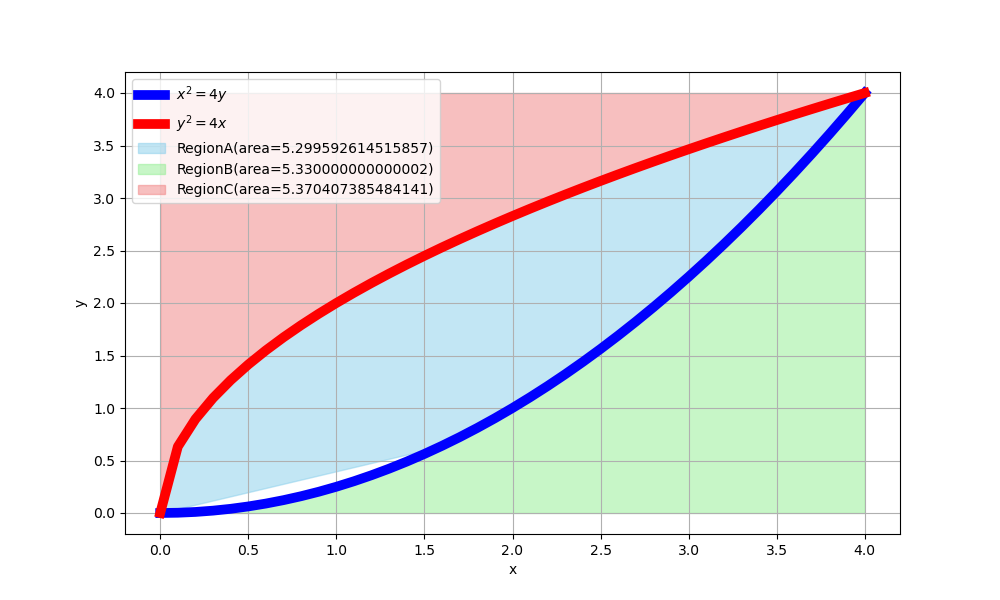
\includegraphics[width=1\columnwidth]{figs/Q3.png}
\end{figure}
\end{document}
\end{document}

